\documentclass{purdue-slide}

% For filler text:
\usepackage[base]{babel}
\usepackage{lipsum}
\usepackage{lmodern}
\usepackage{pgfplots}
\usepackage{caption}
\usepackage{tikz}
\usepackage{booktabs, makecell}
\usepackage{minted}
\usetikzlibrary{positioning}

\usepackage{xcolor} % for colors

% --- Minted Configuration for Beamer ---
% This setup helps fit code onto slides and makes it readable.
\setminted{
	fontsize=\tiny, % Or \small, \scriptsize depending on your needs
	baselinestretch=1.1,   % Adjust line spacing
	breaklines=true,       % Crucial for long lines on slides
	breakafter=-_,          % Allow breaks after hyphens and underscores
	frame=lines,           % Adds a light frame around the code
	framesep=2mm,          % Padding around the frame
	bgcolor=bgcode,        % Background color for the code block
	highlightcolor=hlline, % Color for highlighted lines (if using highlightlines)
	linenos=false,         % Set to true for line numbers
	tabsize=4,
	gobble=0               % Removes leading whitespace (e.g. if code is indented in .tex)
}

% Define custom colors for minted background (optional, but nice for slides)
\definecolor{bgcode}{rgb}{0.95,0.95,0.95} % A light gray
\definecolor{hlline}{rgb}{0.9,0.9,0.9}    % A slightly darker gray for highlighted lines

\author{Stan Ioan-Victor, Ioan-Gabriel Spatariu, Ana Sabina Tatar, Mihnea-Gabriel Vasile, Tepfenhart Bertold }
% Add comment

\begin{document}

\begin{titleframe}{PuLP with Python}
	\subtitle{Solving MILP problems using the GLPK solver.}
	\maketitle
\end{titleframe}

\begin{frame}{Contents}
	% \textbf{Introduction to Linear Programming} \\
	% \textbf{Mathematical Theory \& Theorems} \\
	% \textbf{Introduction to PuLP} \\
	% \textbf{Case Studies} \\
	% \textbf{Resources \& References} \\
	\tableofcontents
\end{frame}

\section{Theoretical Foundation (Ionut)}

\begin{frame}{Fundamental Theorem of LP}
	\textbf{Theorem:} If a linear programming (LP) problem is feasible and bounded, then it has an optimal solution.
\end{frame}

\begin{frame}{Proof of the Theorem}
	Without loss of generality, we may assume that the LP problem is of the form:
	\[
		\begin{aligned}
			& \min \mathbf{c}^\top \mathbf{x} \\
			(P) \quad & \text{s.t. } A\mathbf{x} \geq \mathbf{b}
		\end{aligned}
	\]
	where $m$ and $n$ are positive integers,  $A \in \mathbb{R}^{m \times n}, \ \mathbf{b} \in \mathbb{R}^m, \mathbf{c} \in \mathbb{R}^n,$ $ \text{ and }
	\mathbf{x} =
	\begin{bmatrix}
		x_1 \\
		\vdots \\
		x_n
	\end{bmatrix} \text{ is a tuple of variables. }$

\end{frame}

\begin{frame}{Transforming to Standard Form}
	\quad Any LP problem can be converted to the standard form $(P)$ having the same feasible region and optimal solution set.

	For this, note that:

	\begin{itemize}
		\item Constraints of the form $\mathbf{a}^\top \mathbf{x} \leq \beta$ become $-\mathbf{a}^\top \mathbf{x} \geq -\beta$
		\item Constraints of the form  $\mathbf{a}^\top \mathbf{x} = \beta$ become:
			\[
    \mathbf{a}^\top \mathbf{x} \geq \beta \quad \text{and} \quad -\mathbf{a}^\top \mathbf{x} \leq -\beta
			\]
		\item Maximization problems become minimizations of $-\mathbf{c}^\top \mathbf{x}$
	\end{itemize}
\end{frame}

\begin{frame}{Auxiliary System}
	Suppose $(P)$ is feasible. Define an auxiliary system:
	\[
		(S) \quad
		\begin{cases}
			z - \mathbf{c}^\top \mathbf{x} \geq 0 \\
			-z + \mathbf{c}^\top \mathbf{x} \geq 0 \\
			A\mathbf{x} \geq \mathbf{b}
		\end{cases}
	\]

	\vspace{0.5em}
	Solving $(P)$ is equivalent to minimizing $z$ in $(S)$.

	\vspace{0.5em}
	We eliminate variables $x_1, \dots, x_n$, reducing $(S)$ to a system $(S')$ involving only $z$.
\end{frame}

\begin{frame}{Boundedness and Optimal Solution}
	If $(P)$ is bounded, then $(S')$ must include the constraints:
	\[
		z \geq \beta_i \text{, where } \beta_i \in \mathbb{R}, \forall  i = 1, \dots, p, \text{ with } p \in \mathbf{N^*}.
	\]
	Define $\gamma = \max\{\beta_1, \dots, \beta_p\}$. Then for any solution $x, z$ to $(S)$, $z$ is at least $\gamma$. But we can set $z = \gamma$ and extend it to a solution for $(S)$.

	Hence, we obtain an optimal solution for $(P)$ and $\gamma$ is the optimal value. This completes the proof of the theorem.
\end{frame}

\section{Hand-written examples (Ana)}

\begin{titleframe}{Hand-written Examples}

\end{titleframe}

\begin{frame}{LP Problem: Maximize Workshop Profit}
	A workshop produces:
	\begin{itemize}
		\item Desks: 4h woodworking, 2h painting, \$40 profit
		\item Chairs: 3h woodworking, 1h painting, \$25 profit
	\end{itemize}

	Available resources:
	\begin{itemize}
		\item 24 hours of woodworking
		\item 10 hours of painting
	\end{itemize}

	\textbf{Goal:} Maximize profit by choosing how many desks and chairs to build.
\end{frame}

\begin{frame}{LP Formulation}
	Let:
	\begin{itemize}
		\item \(x\): number of desks
		\item \(y\): number of chairs
	\end{itemize}

	\textbf{Maximize: } \(Z = 40x + 25y\)

	\textbf{Subject to:}
	\[
		\begin{aligned}
			4x + 3y &\leq 24 \quad \text{(woodworking)} \\
			2x + y &\leq 10 \quad \text{(painting)} \\
			x, y &\geq 0
		\end{aligned}
	\]
\end{frame}

\begin{frame}{LP Solution by Hand: Find Intersection}
	\textbf{Find where constraints intersect:}

	\[
		\begin{aligned}
			4x + 3y &= 24 \\
			2x + y &= 10 \Rightarrow y = 10 - 2x
		\end{aligned}
	\]

	Substitute into the first equation:

	\[
		4x + 3(10 - 2x) = 24 \Rightarrow 4x + 30 - 6x = 24 \Rightarrow -2x = -6 \Rightarrow x = 3
	\]

	Then:

	\[
		y = 10 - 2(3) = 4
	\]

	\textbf{Intersection point: } \((3, 4)\)
\end{frame}

\begin{frame}{LP Solution by Hand: Evaluate Z}
	\textbf{Corner points:}
	\begin{itemize}
		\item \((0, 8)\): \(Z = 0 + 25 \times 8 = 200\)
		\item \((5, 0)\): \(Z = 40 \times 5 + 0 = 200\)
		\item \((3, 4)\): \(Z = 40 \times 3 + 25 \times 4 = 220\) ✅
	\end{itemize}

	\begin{alertblock}{Optimal Solution}
		\(x = 3\), \(y = 4\); Max profit = \textbf{\$220}
	\end{alertblock}
\end{frame}

% Plot
\begin{frame}{Feasible Region: LP - Workshop}
	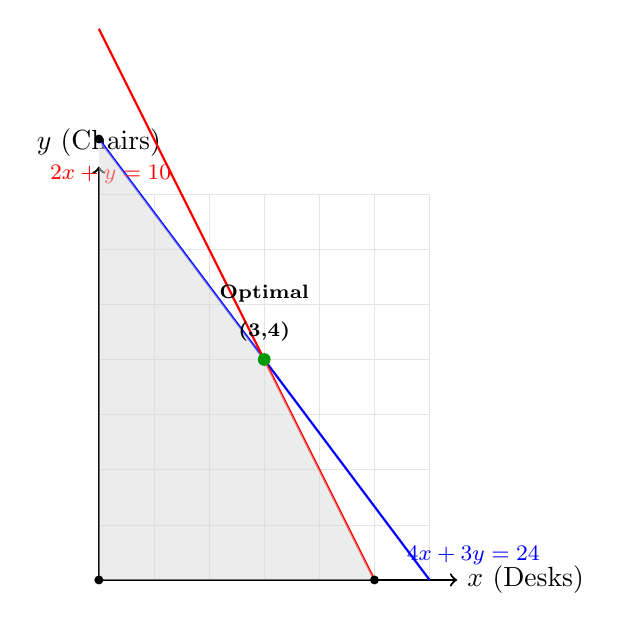
\begin{tikzpicture}[scale=0.7]
		\draw[very thin, gray!20] (0,0) grid (6,7);

		% Axes
		\draw[->, thick] (0,0) -- (6.5,0) node[right] {$x$ (Desks)};
		\draw[->, thick] (0,0) -- (0,7.5) node[above] {$y$ (Chairs)};

		% Constraint lines with adjusted labels
		\draw[thick, blue] (0,8) -- (6,0)
		node[pos=0.9, below right, text=blue] {\footnotesize $4x + 3y = 24$};
		\draw[thick, red] (0,10) -- (5,0)
		node[pos=0.3, above left, text=red] {\footnotesize $2x + y = 10$};

		% Feasible region (shaded)
		\fill[gray!30, opacity=0.5] (0,0) -- (0,8) -- (3,4) -- (5,0) -- cycle;

		% Points
		\foreach \x/\y in {0/0, 0/8, 3/4, 5/0} {
			\filldraw[black] (\x,\y) circle (2pt);
		}

		\node at (3,4.5) {\scriptsize \textbf{(3,4)}};
		\filldraw[green!60!black] (3,4) circle (3pt);
		\node at (3,5.2) {\scriptsize \textbf{Optimal}};
	\end{tikzpicture}
	\vspace{-1em}
	\captionof{figure}{Feasible region for LP: Maximize \$40x + \$25y}
\end{frame}

\begin{frame}{ILP Problem: Integer Optimization}
	\textbf{Objective:} Maximize \(Z = 3x + 2y\)

	\textbf{Subject to:}
	\[
		\begin{aligned}
			x + y &\leq 4 \\
			2x + y &\leq 5 \\
			x, y &\in \mathbb{Z}_{\geq 0}
		\end{aligned}
	\]

	\textbf{Step 1: Find feasible integer pairs \((x,y)\):}
	\begin{itemize}
		\item Try values: \((0,0)\), \((1,2)\), \((2,1)\), \((1,3)\), etc.
	\end{itemize}

	\textbf{Step 2: Evaluate \(Z = 3x + 2y\)}

	\begin{itemize}
		\item \((1,3) \Rightarrow Z = 9\) ✅
		\item \((2,1) \Rightarrow Z = 8\)
		\item \((0,4) \Rightarrow Z = 8\)
	\end{itemize}

	\begin{alertblock}{Optimal ILP Solution}
		\(x = 1\), \(y = 3\); Max value = \textbf{9}
	\end{alertblock}
\end{frame}

\begin{frame}{ILP Solution by Hand}
	\textbf{Step 1: Generate integer pairs \((x, y)\) that satisfy the constraints.}

	\textbf{Constraints:}
	\[
		\begin{aligned}
			x + y &\leq 4 \\
			2x + y &\leq 5 \\
			x, y &\in \mathbb{Z}_{\geq 0}
		\end{aligned}
	\]

	Try values of \(x\) from 0 to 3:

	\begin{itemize}
		\item \(x = 0\): \(y \leq 4\) and \(y \leq 5\) → \(y = 0,1,2,3,4\)
		\item \(x = 1\): \(y \leq 3\) and \(y \leq 3\) → \(y = 0,1,2,3\)
		\item \(x = 2\): \(y \leq 2\) and \(y \leq 1\) → \(y = 0,1\)
		\item \(x = 3\): \(y \leq 1\) and \(y \leq -1\) → ❌ infeasible
	\end{itemize}

	Total valid integer points:
	\((0,0), (0,1), (0,2), (0,3), (0,4), (1,0), (1,1), (1,2), (1,3), (2,0), (2,1)\)
\end{frame}

\begin{frame}{Feasible Integer Points: ILP}
	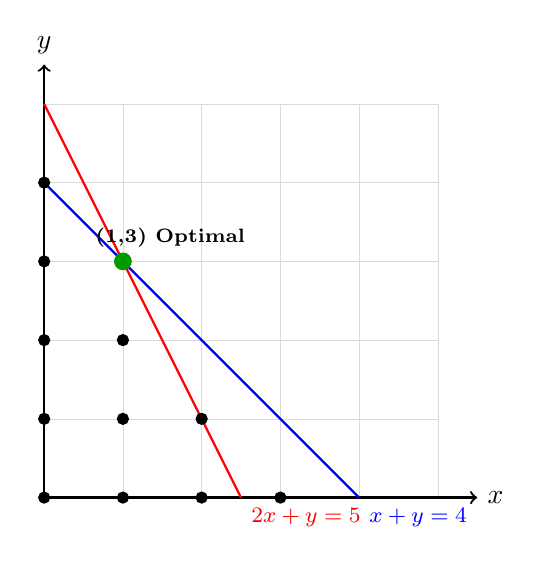
\begin{tikzpicture}[scale=1]
		\draw[very thin, gray!30] (0,0) grid (5,5);

		% Axes
		\draw[->, thick] (0,0) -- (5.5,0) node[right] {$x$};
		\draw[->, thick] (0,0) -- (0,5.5) node[above] {$y$};

		% Constraint lines
		\draw[thick, blue] (0,4) -- (4,0) node[below right] {\footnotesize $x + y = 4$};
		\draw[thick, red] (0,5) -- (2.5,0) node[below right] {\footnotesize $2x + y = 5$};

		% Feasible integer points
		\foreach \x/\y in {
			0/0, 0/1, 0/2, 0/3, 0/4,
			1/0, 1/1, 1/2, 1/3,
			2/0, 2/1,
			3/0
		} {
			\filldraw[black] (\x,\y) circle (2pt);
		}

		% Optimal point
		\filldraw[green!60!black] (1,3) circle (3pt);
		\node at (1.6,3.3) {\scriptsize \textbf{(1,3) Optimal}};
	\end{tikzpicture}
	\captionof{figure}{Feasible integer points for ILP: Maximize \(3x + 2y\)}
\end{frame}

\section{Introduction to PuLP and GLPK (Vic)}

\begin{titleframe}{Introduction to PuLP and GLPK}
	\textbf{PuLP} is a Python modeler for mixed-integer linear programming (MILP) problems. It is used to first phrase the question and it produces LP and MPS files from your problem statement. Then a solver like \textbf{GLPK} comes in and actually solves the problem.
\end{titleframe}

\begin{frame}[fragile]{Intro}

	While I admit this is taken straight from the documentation, I can't think of anything better as of now.
	If we want to restrain a variable between $0 \leq x \leq 3$
	\begin{minted}{python3}
from pulp import *
x = LpVariable("x", 0, 3)	
	\end{minted}
	but if we want a discrete, binary value:
\begin{minted}{python3}
y = LpVariable("y", cat="Binary")
\end{minted}
	Generally \textbf{defining} new problems is done with
\begin{minted}{python3}
prob = LpProblem("myProblem", LpMinimize)
\end{minted}

	and adding constraints is as easy as
\begin{minted}{python3}
prob += x + y <= 2
\end{minted}

\end{frame}

\begin{frame}[fragile]{Solvers}
	\textbf{ Solving } problems is done with a quick	
\begin{minted}{python3}
status = prob.solve()
\end{minted}
	To just us the included, built-in solver, namely \verb|CBC| (About
	COIN-OR Branch-and-Cut)
	But one can also specify
\begin{minted}{python3}
status = prob.solve(GLPK(msg = 0))
\end{minted}
	specifically, and getting the values for our solved variables:
\begin{minted}{python3}
value(y)
>3.0
value(x)
>3.0
\end{minted}
	But that's of course granted if \verb|LpStatus[status]| is 'Optimal' out of the possible \verb|“Undefined”, “Unbounded”, “Infeasible”, “Not Solved”|
\end{frame}

\begin{frame}[fragile]{Independently solving}
	We can also, as mentioned previously prompt	PuLP to write the problem to an external \verb|.lp| file, so for a problem of the type
	\begin{minted}{python3}
from pulp import *

prob = LpProblem("SimpleProblem", LpMinimize)

# Define variables
x = LpVariable("x", lowBound=0)
y = LpVariable("y", lowBound=0)

# Obj function
prob += 3 * x + 2 * y, "TotalCost"

# Constraints
prob += 2 * x + y >= 8
prob += x + 2 * y >= 6

prob.writeLP("simple_problem.lp")	
	\end{minted}
	"\verb|simple_problem.lp|" would contain:
\end{frame}

\begin{frame}[fragile]{simpleproblem.lp}
	\begin{minted}{texcomments}
Minimize
  TotalCost: 3 x + 2 y
Subject To
  Constraint1: 2 x + y >= 8
  Constraint2: x + 2 y >= 6
Bounds
  x >= 0
  y >= 0
End	
	\end{minted}
	Then we can call \textbf{GLPK independently}
	\begin{minted}{showspaces}
glpsol --lp simple_problem.lp -o output.sol	
	\end{minted}
	Whose output would be:
\end{frame}

\begin{frame}[fragile]{output.sol}
\begin{minted}{texcomments}
Problem:    simple_problem
Rows:       3
Columns:    2
Non-zeros:  4
Status:     OPTIMAL
Objective:  TotalCost = 9.6 (MINimum)

   No.   Row name        Activity     Lower bound   Upper bound
------ ------------    ------------- ------------- -------------
     1 Constraint1               8.0             8
     2 Constraint2               6.0             6
     3 TotalCost                 9.6

   No. Column name      Activity     Lower bound   Upper bound
------ ------------    ------------- ------------- -------------
     1 x                        2.8             0
     2 y                        1.6             0	
\end{minted}	
\end{frame}

\section{Real World Applications (Bertold)}

\begin{titleframe}{Real World Applications}
	\textbf{Case Study: Blending Problem in Pet Food Production}
\end{titleframe}

\begin{frame}{(MILP) Blending Problem: Whiskas Cat Food}
	So, as a first MILP problem, we've
	got a blending problem —
	basically, we want to make
	Whiskas cat food as cheap as
	possible while still hitting the
	nutrition targets on the label. We
	can play around with how much
	chicken, beef, mutton, rice, wheat,
	and gel to use to make that
	happen.

	\begin{figure}[H]
		\centering
		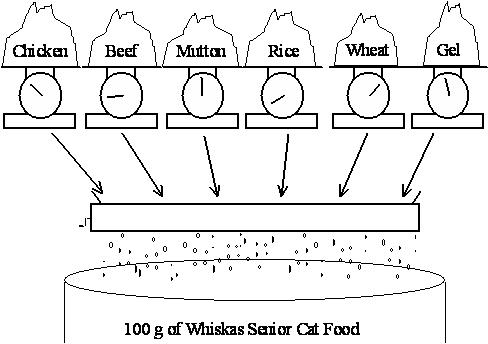
\includegraphics[width=0.4\textwidth]{pics/whiskas_blend_intro.jpg}
		\caption{Whiskas Cat Food}
	\end{figure}
\end{frame}

\begin{frame}{Blending Problem: Whiskas Cat Food}
	\textbf{Objective:} Minimize cost while meeting nutritional requirements.

	\bigskip

	\textbf{Ingredients:} Chicken, Beef, Mutton, Rice, Wheat bran, Gel

	\bigskip

	The costs of the ingredients per gram are as follows:
	\begin{itemize}
		\item Chicken: \$0.013
		\item Beef: \$0.008
		\item Mutton: \$0.010
		\item Rice: \$0.002
		\item Wheat: \$0.005
		\item Gel: \$0.001
	\end{itemize}

	For this exercise, we will ignore the vitamin and mineral ingredients, as their costs are likely negligible.
\end{frame}

\begin{frame}{Nutritional Data (per gram)}
	\centering
	\begin{tabular}{lcccc}
		\toprule
		Ingredient & Protein & Fat & Fibre & Salt \\
		\midrule
		Chicken     & 0.100 & 0.080 & 0.001 & 0.002 \\
		Beef        & 0.200 & 0.100 & 0.005 & 0.005 \\
		Mutton      & 0.150 & 0.110 & 0.003 & 0.007 \\
		Rice        & 0.000 & 0.010 & 0.100 & 0.002 \\
		Wheat bran  & 0.040 & 0.010 & 0.150 & 0.008 \\
		Gel         & 0.000 & 0.000 & 0.000 & 0.000 \\
		\bottomrule
	\end{tabular}
\end{frame}

\begin{frame}{Simplified Formulation}
	\textbf{Variables:}
	\[
		x_1 = \% \text{Chicken}, \quad x_2 = \% \text{Beef}
	\]

	\textbf{Objective:}
	\[
		\min\ 0.013x_1 + 0.008x_2
	\]

	\textbf{Constraints:}
	\begin{align*}
		1.0x_1 + 1.0x_2 &= 100 \\
		0.1x_1 + 0.2x_2 &\ge 8.0 \quad \text{(Protein)} \\
		0.08x_1 + 0.1x_2 &\ge 6.0 \quad \text{(Fat)} \\
		0.001x_1 + 0.005x_2 &\le 2.0 \quad \text{(Fibre)} \\
		0.002x_1 + 0.005x_2 &\le 0.4 \quad \text{(Salt)}
	\end{align*}
\end{frame}

\begin{frame}[fragile]{Python Code}

	\begin{minted}{python}
from pulp import *
prob = LpProblem("The Whiskas Problem", LpMinimize)

x1 = LpVariable("ChickenPercent", 0, None, LpInteger)
x2 = LpVariable("BeefPercent", 0)

prob += 0.013 * x1 + 0.008 * x2, "Total Cost of Ingredients per can"
prob += x1 + x2 == 100, "PercentagesSum"

prob += 0.100 * x1 + 0.200 * x2 >= 8.0, "ProteinRequirement"
prob += 0.080 * x1 + 0.100 * x2 >= 6.0, "FatRequirement"
prob += 0.001 * x1 + 0.005 * x2 <= 2.0, "FibreRequirement"
prob += 0.002 * x1 + 0.005 * x2 <= 0.4, "SaltRequirement"

prob.writeLP("WhiskasModel.lp")
print("Status:", LpStatus[prob.status])

for v in prob.variables():
	print(v.name, "=", v.varValue)

print("Total Cost of Ingredients per can = ", value(prob.objective))
\end{minted}

\end{frame}

\begin{frame}{Solution Results}
	\textbf{Simplified Model:}
	\begin{itemize}
		\item Chicken: 33.33\%
		\item Beef: 66.67\%
		\item Cost per can: \$0.96
	\end{itemize}

	\bigskip

	\textbf{Full Model (All 6 Ingredients):}
	\begin{itemize}
		\item Beef: 60\%
		\item Gel: 40\%
		\item Cost per can: \$0.52
	\end{itemize}
\end{frame}

\begin{frame}[fragile]{Full solution}
    \begin{minted}{python3}
from pulp import *
Ingredients = ["CHICKEN", "BEEF", "MUTTON", "RICE",
"WHEAT", "GEL"]
costs = {
	"CHICKEN": 0.013,
	"BEEF": 0.008,
	"MUTTON": 0.010,
	"RICE": 0.002,
	"WHEAT": 0.005,
	"GEL": 0.001,
}
proteinPercent = {
	"CHICKEN": 0.100,
	"BEEF": 0.200,
	"MUTTON": 0.150,
	"RICE": 0.000,
	"WHEAT": 0.040,
	"GEL": 0.000,
}
    \end{minted}
\end{frame}

\begin{frame}[fragile,plain]
	\begin{minted}{python3}
fatPercent = {
	"CHICKEN": 0.080,
	"BEEF": 0.100,
	"MUTTON": 0.110,
	"RICE": 0.010,
	"WHEAT": 0.010,
	"GEL": 0.000,
}
fibrePercent = {
	"CHICKEN": 0.001,
	"BEEF": 0.005,
	"MUTTON": 0.003,
	"RICE": 0.100,
	"WHEAT": 0.150,
	"GEL": 0.000,
}
saltPercent = {
	"CHICKEN": 0.002,
	"BEEF": 0.005,
	"MUTTON": 0.007,
	"RICE": 0.002,
	"WHEAT": 0.008,
	"GEL": 0.000,
}
	\end{minted}
\end{frame}

\begin{frame}[fragile,plain]
	\begin{minted}{python3}
prob = LpProblem("The Whiskas Problem", LpMinimize)
ingredient_vars = LpVariable.dicts("Ingr", Ingredients, 0)
prob += (
lpSum([costs[i] * ingredient_vars[i] for i in Ingredients]),
"Total Cost of Ingredients per can",
)
prob += lpSum([ingredient_vars[i] for i in Ingredients]) == 100, "PercentagesSum"
prob += (
lpSum([proteinPercent[i] * ingredient_vars[i] for i in Ingredients]) >= 8.0,
"ProteinRequirement",
)
prob += (
lpSum([fatPercent[i] * ingredient_vars[i] for i in Ingredients]) >= 6.0,
"FatRequirement",
)
prob += (
lpSum([fibrePercent[i] * ingredient_vars[i] for i in Ingredients]) <= 2.0,
"FibreRequirement",
)
prob += (
lpSum([saltPercent[i] * ingredient_vars[i] for i in Ingredients]) <= 0.4,
"SaltRequirement",
)
prob.writeLP("WhiskasModel2.lp")
prob.solve()
print("Status:", LpStatus[prob.status])
for v in prob.variables():
print(v.name, "=", v.varValue)
print("Total Cost of Ingrediets per can = ", value(prob.objective))
	\end{minted}
\end{frame}

\begin{frame}{Execution Time of previous code}
	\begin{figure}[H]
		\centering
		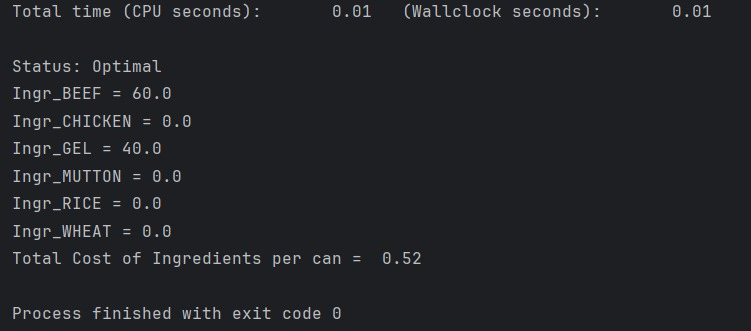
\includegraphics[width=340pt]{pics/bertold-rez-2-exec-time.jpeg}
	\end{figure}
\end{frame}

\section{A Transportation Problem (Mihnea)}

\begin{titleframe}{Case Study: A Transportation Problem}

\end{titleframe}

\begin{frame}{A Transportation Problem: Introduction}
	\textbf{Scenario:} A boutique brewery distributes beer from its warehouses to several bars.
	\begin{itemize}
		\item The brewery has two warehouses (A and B) and serves five bars (1, 2, 3, 4, 5).
		\item Each week, bars submit orders for a specific number of beer crates.
		\item \textbf{Objective:} Determine the optimal shipment plan from warehouses to bars to minimize total transportation costs for the entire operation.
		\item \textbf{Example Data for a Week:}
			\begin{itemize}
				\item Warehouse A supply: 1000 cases
				\item Warehouse B supply: 4000 cases
				\item Bar demands: 500 (Bar 1), 900 (Bar 2), 1800 (Bar 3), 200 (Bar 4), 700 (Bar 5) cases.
			\end{itemize}
	\end{itemize}
\end{frame}

%-----------------------------------------------------------------------------------------

\begin{frame}{Problem Formulation}
	\textbf{Decision Variables:}
	\begin{itemize}
		\item Let $x(w,b)$ be the number of crates of beer to ship from warehouse $w$ to bar $b$.
		\item These variables must be non-negative integers ($x(w,b) \ge 0$).
	\end{itemize}

	\textbf{Objective Function:} Minimize total transportation costs.
	\begin{itemize}
		\item Assume a fixed cost per crate for each warehouse-to-bar route.
		\item Example Costs (\$/crate):
			\tiny
			\begin{center}
				\begin{tabular}{lccccc}
					\toprule
					From Warehouse & Bar 1 & Bar 2 & Bar 3 & Bar 4 & Bar 5 \\
					\midrule
					A & 2 & 4 & 5 & 2 & 1 \\
					B & 3 & 1 & 3 & 2 & 3 \\
					\bottomrule
				\end{tabular}
			\end{center}
			\normalsize
		\item Minimize: $\sum_{w \in \text{Warehouses}} \sum_{b \in \text{Bars}} \text{cost}(w,b) \cdot x(w,b)$
	\end{itemize}
\end{frame}

\begin{frame}{Constraints}
	\begin{itemize}
		\item \textbf{Supply Constraints:} The total beer shipped from each warehouse cannot exceed its supply.
			\begin{itemize}
				\item E.g., For Warehouse A: $\sum_{b \in \text{Bars}} x(A,b) \leq 1000$
			\end{itemize}
		\item \textbf{Demand Constraints:} The total beer received by each bar must be at least its demand.
			\begin{itemize}
				\item E.g., For Bar 1: $\sum_{w \in \text{Warehouses}} x(w,1) \geq 500$
			\end{itemize}
	\end{itemize}
\end{frame}

%-----------------------------------------------------------------------------------------

\begin{frame}[fragile]{PuLP Model Highlights}
	\textbf{1. Define Nodes and Data Structures:}
\begin{minted}{python3}
Warehouses = ["A", "B"]
Bars = ["1", "2", "3", "4", "5"]
supply = {"A": 1000, "B": 4000}
demand = {"1": 500, "2": 900, "3": 1800, "4": 200, "5": 700}
costs = makeDict([Warehouses, Bars], cost_data, 0)	#cost matrix, converted to PulP dictionary
\end{minted}

	\textbf{2. Create Problem and Variables:}
	\begin{minted}{python3}
prob = LpProblem("Beer Distribution", LpMinimize)
vars =
LpVariable.dicts("Route", (Warehouses, Bars), 0, None, LpInteger)
	\end{minted}
\end{frame}

\begin{frame}[fragile]{3. Add Objective Function and Constraints}
	\begin{minted}{python3}
		prob += lpSum([vars[w][b] * costs[w][b] for (w,b) in Routes]), "Total Cost"#Objective function
		prob += lpSum([vars[w][b] for b in Bars]) <= supply[w] # Supply constraints
		prob += lpSum([vars[w][b] for w in Warehouses]) >= demand[b], f"Demand_{b}" # Demand constraints
	\end{minted}
	The problem is then solved using prob.solve().
\end{frame}

%-----------------------------------------------------------------------------------------

\begin{frame}{Extensions and Solution Insights}
	\textbf{Balancing the Problem:}
	\begin{itemize}
		\item Transportation problems are often "balanced" (total supply = total demand).
		\item \textbf{Excess Supply:} If supply > demand (like in the example: 5000 cases supply vs 4100 demand ), a "dummy demand node" can be added.
			\begin{itemize}
				\item The "cost" of shipping to this dummy node represents storage costs (can be zero if not applicable).
				\item Demand for the dummy node = Total Supply - Total Real Demand (e.g., 900 cases).
			\end{itemize}
		\item \textbf{Excess Demand:} If demand > supply, a "dummy supply node" can balance the problem.
			\begin{itemize}
				\item This is crucial because an unbalanced problem with excess demand is infeasible.
				\item The "cost" from the dummy supply can represent penalties for unmet demand or cost of acquiring from alternative sources.
			\end{itemize}
	\end{itemize}
\end{frame}

\begin{frame}{Nature of Solution}
	\begin{itemize}
		\item If supply and demand values are integers, the LP solution to the transportation problem will inherently be integer values.  (Though variables are often explicitly defined as `LpInteger` in PuLP for clarity/mixed-integer problems).
	\end{itemize}

	\textbf{Presenting the Solution:}
	\begin{itemize}
		\item Typically includes a list of non-zero shipments, total cost, and a management summary.
	\end{itemize}
\end{frame}

\end{document}